\chapter{Edge Contraction}
\label{ch:graphcon::edge}

\begin{preamble}
This section describes the edge partition and edge contraction.
%
Edge contraction is an instance of a graph-contraction where blocks
being contracted correspond to edges.
\end{preamble}


\section{Edge Partition}
\label{sec:graphcon::edge::partition}

\begin{flex}

\begin{definition}[Edge Partition]
\label{def:graphcon::edge::edge-partition}
An~\defn{edge partition} is a 
%
\href{def:graphcon::intro::prelim::graph-partition}{graph partition}
%
where each block is either a single vertex or two vertices connected
by an edge.
%
\end{definition}

\begin{example}
\label{ex:graphcon::edge-partition}
An example edge partition in which every block consists of two
vertices and an edge between them. 
\begin{center}
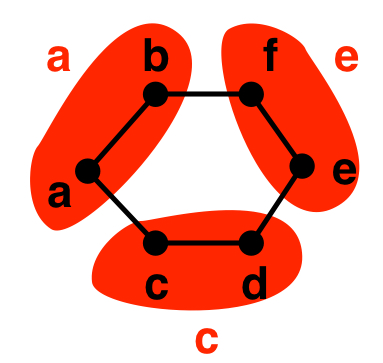
\includegraphics[width=2.0in]{./graph-contraction/media-edge/edge-partition-example-1.jpg}
\end{center}
\end{example}

%% \begin{note}
%% In edge contraction, blocks cannot be just pairs of vertices, because
%% the graph might not have an even number of vertices.
%% %
%% Even when the graph does have an even number of vertices (no pun
%% intended), it might not by possible to partition it into blocks where
%% each block is an edge.
%% \end{note}

\end{flex}

\begin{flex}
\begin{exercise}
Give an example graph whose edge partitions always contain a block
that consists of a single vertex.
\end{exercise}

\begin{solution}
Any graph which has an isolated vertex, i.e., a vertex with no
incident edges would work.
\end{solution}
\end{flex}

\begin{gram}[Edge Partitions and Vertex Matching]
%
%% \begin{teachask}
%% How can we construct an edge-partitioning in the general case?
%% \end{teachask}
%
Finding an edge partition of a graph is closely related to the
problem of finding an independent edge set or a vertex matching.
%
A vertex matching in  a graph is a subset of the edges that do not share an endpoint, i.e., no two edges are incident on the same vertex.
%
We can construct an edge partition from a vertex matching by
constructing a block for each edge in the matching and placing all the
remaining vertices into their own singleton blocks.
\end{gram}


\begin{flex}
\begin{definition}[Vertex Matching]
\label{def:graphcon::edge::vertex-matching}
A~\defn{vertex matching} for an undirected graph $G = (V,E)$ is a
subset of edges $M \subseteq E$ such that no two edges in $M$ are
incident on the same vertex. In other words, each vertex in $M$ have
degree at most $1$. 

The problem of finding the largest vertex matching for a graph is
called the~\defn{maximum vertex matching} problem.  
\end{definition}

\begin{gram}[Algorithms for Maximum Vertex Matching]
Maximum Vertex Matching is a well-studied problem and many algorithms
have been proposed, including one that can solve the problem in
$O(\sqrt{|V|}|E|)$ work.
\end{gram}


\begin{example}[Vertex Matching]
\label{ex:graphcon::edge::vertex-matching}
A vertex matching for a graph (highlighted edges) and the
corresponding blocks.
\begin{center}
  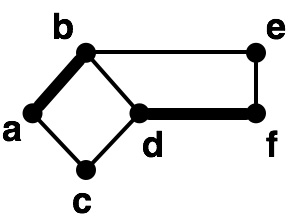
\includegraphics[width=2in]{./graph-contraction/media-edge/matching-example.jpg}
\hspace{1in}
  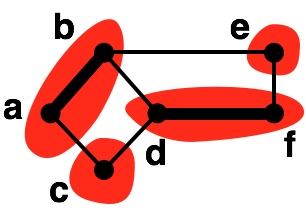
\includegraphics[width=2in]{./graph-contraction/media-edge/matching-example-partitioned.jpg}
\end{center}

The vertex matching defines four blocks (circled), two of them defined
by the edges in the matching, $\cset{\vname{a},\vname{b}}$ and
$\cset{\vname{d},\vname{f}}$, and two of them are the unmatched
vertices $\vname{c}$ and $\vname{e}.$
\end{example}
\end{flex}

\begin{note}
For edge contraction, we do not need a maximum matching but one that
it is sufficiently large.
%
\end{note}

\begin{algorithm}[Greedy Vertex Matching]
\label{alg:graphcon::edge::greedy-matching}
We can use a greedy algorithm to construct a vertex matching by
iterating over the edges while maintaining an initially empty
matching~$M$.
%
The greedy algorithm considers each edge and proceeds as follows:
\begin{itemize}
\item if no edge in $M$ is already incident on its endpoints, then the
  algorithm adds the edge to $M$,

\item otherwise,  the algorithm tosses away the edge.
\end{itemize}
\end{algorithm}

\begin{flex}
\begin{exercise}
Does the greedy vertex matching algorithm always returns a maximum
vertex matching?
\end{exercise}
\begin{solution}
No.
\end{solution}
\end{flex}

\begin{exercise}
Prove that the greedy algorithm finds a solution within a factor two
of optimal.
\end{exercise}

\begin{flex}
\begin{exercise}
Is the greedy algorithm parallel?
\end{exercise}
\begin{solution}
The greedy algorithm is sequential, because each decision depends on
previous decisions.
\end{solution}
\end{flex}



%% %
%% \begin{teachask}
%% Describe a parallel algorithm for  vertex matching?
%% \end{teachask}
%% %

\begin{gram}[Randomized Symmetry Breaking]
To find a 
%
\href{def:graphcon::edge::vertex-matching}{vertex matching}
%
in parallel, we want to make local and parallel decisions at each vertex independent of other vertices.  
%
One possibility is for each vertex to select one of its neighbors
arbitrarily but in some deterministic fashion.
%
Such a selection can be made in parallel but there is one problem:
multiple vertices might select the same vertex to match with.
%

We therefore need a way to \emph{break the symmetry} that arises when
two vertices try to match with the same vertex.
%% %
%% \begin{teachask}
%% Can you use randomization to break the symmetry? 
%% \end{teachask}
%% %
To this end, we can use randomization.
%
There are several different ways to use randomization but they are all essentially the same and yield the same bounds with a constant factor.
\end{gram}


\begin{flex}
\begin{algorithm}[Parallel Vertex Matching]
\label{alg:graphcon::edge::parallel-matching}
To compute a vertex matching the
%
\defn{parallel vertex matching algorithm}
%
flips a coin for each edge in parallel.
%
The algorithm then selects an edge $(u, v)$ and matches $u$ and $v$,
if the coin for the edge comes up heads and all the edges incident on
$u$ and $v$ flip tails.  
%
\end{algorithm}

\begin{example}[Parallel Vertex Matching]
An example run of he parallel vertex matching algorithm.
 
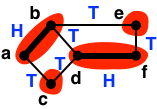
\includegraphics[width=2in]{./graph-contraction/media-edge/vertex-matching-randomized.jpg}
\end{example}
\end{flex}

\begin{exercise}
Prove that the algorithm produces a vertex matching, i.e., it
guarantees that a vertex is matched with at most one other vertex.
\end{exercise}


\subsection{Analysis of Parallel Edge Partition}
\label{sec:edge::partition::analysis}

We analyze the effectiveness of the parallel 
%
\href{alg:graphcon::edge::parallel-matching}{edge partition algorithm}
%
in selecting a matching that consists of as many edge blocks
(equivalently as few singleton blocks) as possible.
%
We first consider cycle graphs and then general graphs.


\subsubsection{Cycle Graphs}
\label{sec:edge::partition::analysis::cycle}

\begin{gram}[Probability of Selecting an Edge in a Cycle]
\label{graphcon::edge::analysis::cycle::pr}
We want to determine the probability that an edge is selected in a
cycle, where each vertex has exactly two neighbors. 
%
Because the coins are flipped independently at random, and each vertex
has degree two, the probability that an edge picks heads and its two
adjacent edges pick tails is $\frac{1}{2} \cdot \frac{1}{2} \cdot
\frac{1}{2} = \frac{1}{8}$.
\end{gram}

\begin{example}[Edge Partition of a Cycle] 
\label{ex:graphcon::edge::analysis::cycle::1}
A graph consisting of a single cycle.    
  \begin{center}
  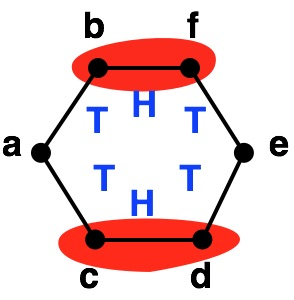
\includegraphics[width=1.5in]{./graph-contraction/media-edge/cycle-graph.jpg}
  \end{center}
Each edge flips a coin that comes up either heads ($H$) or tails
($T$).  
%
We select an edge if it turns up heads and all other edges
incident on its endpoints are tails.  In the example the edges
$\cset{\vname{c},\vname{d}}$ and $\cset{\vname{b},\vname{f}}$ are
selected.
\end{example}


\begin{gram}[Expected Number of Edges Selected]
\label{graphcon::edge::analysis::cycle::exp}
To analyze the number of edges (blocks) selected in expectation, let
$R_e$ be an indicator random variable denoting whether $e$ is selected
or not, that is $R_e = 1$ if $e$ is selected and $0$ otherwise.
Recall that the expectation of indicator random variables is the same
as the probability it has value $1$ (true).  Therefore we have $E[R_e]
= 1/8$.
%
Thus summing over all edges, we conclude that expected number of edges
selected is $\frac{m}{8}$ (note, $m=n$ in a cycle graph). 
%
Thus we conclude that in expectation, a constant fraction
$\left(\frac{1}{8}\right)$ of the edges are selected to be their own blocks.
\end{gram}



\begin{flex}
\begin{exercise}
  Modify the algorithm to improve the expected number of edges selected.
\end{exercise}

\begin{gram}[Improving the Expectation]
\label{graphcon::edge::analysis::cycle::improve}
There are several ways to improve the number of select edges. 
%
One way is for each vertex to pick one of its neighbors and to select
an edge $(u,v)$ if it was picked by both $u$ and $v$.  In the case of
a circle, this increases the expected number of selected edges to
$\frac{m}{4}$.
%

Another way is let each edge pick a random number in some range and
then select and edge if it is the local maximum, i.e., it picked the
highest number among all the edges incident on its end points. This
increases the expected number of selected edges to
$\frac{m}{3}$.
\end{gram}
\end{flex}

\subsubsection{Star Graphs}
\label{sec:graphcon::edge::analysis::star}

\begin{gram}[Limitation of Edge Partition]
\label{graphcon::edge::analysis::star::limitation}
Although our edge partition algorithm works quite well on cycle
graphs,
%or sequentially with the appropriate data structures, 
it does not work well for arbitrary graphs.  The problem is in an edge
partition, only one edge incident on a vertex can be its own block.
%
Therefore if there is a vertex with high degree, then only one of its
edges can be selected.
%
Star graphs are a canonical example of such graphs, although there are
many others.
\end{gram}
%

\begin{flex}
\begin{definition}[Star Graph]
\label{def:graphcon::edge::analysis::star::star-graph}

A~\defn{star graph} $G = (V,E)$ is an undirected graph with 
\begin{itemize}
\item a  ~\defn{center} vertex $v \in V$, and 

\item a set of edges $E$ that attach   $v$ directly to the rest of the vertices, called
 ~\defn{satellites}, i.e., 
$E = \cset{\cset{v,u} : u
    \in V \setminus \cset{v}}$.
\end{itemize}
\end{definition}

\begin{example} 
The following are star graphs:
\begin{itemize}
\item a single vertex, and
\item a single edge.
\end{itemize}
\end{example}
\end{flex}

\section{Edge Contraction}
\label{sec:graphcon::edge::contraction}

\begin{algorithm}[Parallel Edge Contraction]
\label{alg:graphcon::edge::contraction}
Parallel edge contraction algorithm is a specialization of the 
%
\href{def:graphcon::intro::graphcon::technique}{graph contraction technique}
%
that uses the parallel 
%
\href{alg:graphcon::edge::parallel-matching}{vertex matching algorithm}
%
to partition the graph for contraction.
\end{algorithm}

\begin{example}[Edge contraction]
\label{ex:graphcon::edge::contraction::ex1}

An example parallel edge contraction illustrated.

\begin{center}
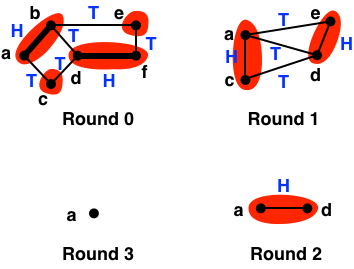
\includegraphics[width=5in]{./graph-contraction/media-edge/edge-contraction-example.jpg}
\end{center}
\end{example}

\begin{gram}[Analysis of Edge Contraction]
The
\href{sec:graphcon::edge::analysis::star}{analysis of edge partition} 
established that using edge partition, we are able to select in
expectation $\frac{1}{8}$ of the edges as their own blocks if the
graph is a cycle.
%
Therefore, after one round of contraction, the number of vertices and
edges in a cycle decrease by an expected constant fraction.
%

In 
%
\href{ch:randomization::select}{randomized algorithms chapter}, 
%
we showed that if each round of an algorithm reduces the size by a
constant fraction in expectation, and if the random choices in the
rounds are independent, then the algorithm will finish in $O(\lg n)$
rounds with high probability. 
%
Recall that all we needed to do is multiply the expected fraction that
remain across rounds and then use Markov's inequality to show that
after some $k \lg n$ rounds the probability that the problem size is a
least $1$ is very small.  
%
For a cycle graph, this technique leads to an
algorithm for graph contraction with linear work and $O(\lg^2{n})$
span.
\end{gram}

\begin{gram}[Analysis for Star Graphs]
Edge contraction works quite poorly on other graphs such as star graphs,
and can result in a partition with many singleton blocks.
%
This is because in an edge partition, only one of the edges incident
on a vertex can be its own block
(\secref{graphcon::edge::analysis::star}),
leading to a poor contraction ratio.
%
Edge contraction therefore is not effective for general graphs.
\end{gram}



%% \begin{teachnote}
%% I (Umut) find the remark below quite confusing. 
%% \end{teachnote}%% \begin{section}
%% \begin{remark}[What is the POINT?]
%% TODO: Maybe expand this into its own subsection 

%%   An abstract data type called disjoint sets is often used to contract
%%   graphs sequentially.  Disjoint sets supply two functions:
%%  ~\defn{union}, which joins two components, and~\defn{find}, which
%%   finds what component a vertex is in.  In our framework, the union
%%   operation is simply edge contraction across a single edge, and the
%%   find is just a lookup in the partition map.  Semantically for a
%%   partition map $P$ we can define $\cd{union}$ as:


%% \[
%% \begin{array}{lcl}
%% ~~\cd{union}~(P,u,v) & = & \{ u' \mapsto~\cd{if}~(v' = u)~\cd{then}~v~\cd{else}~v'
%% \\
 
%%                  & & ~: (u' \mapsto v') \in P \}
%% \end{array}
%% \]

%% where here we have made $v$ the new representative of the super-vertex
%% $\cset{u,v}$, and have updated all vertices that used to point to $u$
%% to now point to $v$.
%% Implementing the $\cd{union}$ this way, however, is inefficient since
%% it can require updating a lot of vertices.  It turns out that the
%% operations can be can be implemented much more efficiently.  Indeed
%% one can implement a data structure that only requires amortized
%% $O(\alpha(n))$ work per operation, where $\alpha(n)$ (the inverse
%% Ackermann function) is a function that is very close ot $O(1)$, and
%% $n$ is the number of operations.
%% \end{remark}
%% \end{section}

